% Source: Code/camera-to-radar_labeller/system_overview.tex
% Description: System architecture. The radar scan feeds through clustering, tracking, and selection before the PTZ camera observes a single blob. Labels propagate back to the track manager.

\documentclass[border=4pt]{standalone}
\usepackage{amsmath,amssymb,amsfonts}
\usepackage{tikz}
\usepackage{xcolor}
\usetikzlibrary{arrows.meta,positioning,calc,patterns,decorations.markings,shapes.geometric,fit,backgrounds}

\definecolor{Garnet}{HTML}{73000A}
\definecolor{Rose}{HTML}{CC2E40}
\definecolor{Atlantic}{HTML}{466A9F}
\definecolor{Congaree}{HTML}{1F414D}
\definecolor{Horseshoe}{HTML}{65780B}
\definecolor{Grass}{HTML}{CED318}
\definecolor{Honeycomb}{HTML}{A49137}
\definecolor{Black90}{HTML}{363636}
\definecolor{Black70}{HTML}{5C5C5C}
\definecolor{Black50}{HTML}{A2A2A2}
\definecolor{Black30}{HTML}{C7C7C7}
\definecolor{Black10}{HTML}{ECECEC}
\definecolor{WarmGrey}{HTML}{676156}
\definecolor{Sandstorm}{HTML}{FFF2E3}

\tikzset{
    every node/.style={font=\small},
    sysblock/.style={
        draw=Congaree, fill=Congaree!10, thick,
        minimum width=2.2cm, minimum height=1cm,
        align=center, sharp corners,
        text=black
    },
    sysarrow/.style={
        -Stealth, thick, color=Garnet
    },
    timeblock/.style={
        draw=none, fill=#1, minimum height=0.5cm,
        sharp corners, text=white, font=\footnotesize\bfseries,
        inner sep=2pt
    },
    ppiblob/.style={
        fill=#1, sharp corners, minimum size=4pt, inner sep=0pt
    },
}

\begin{document}
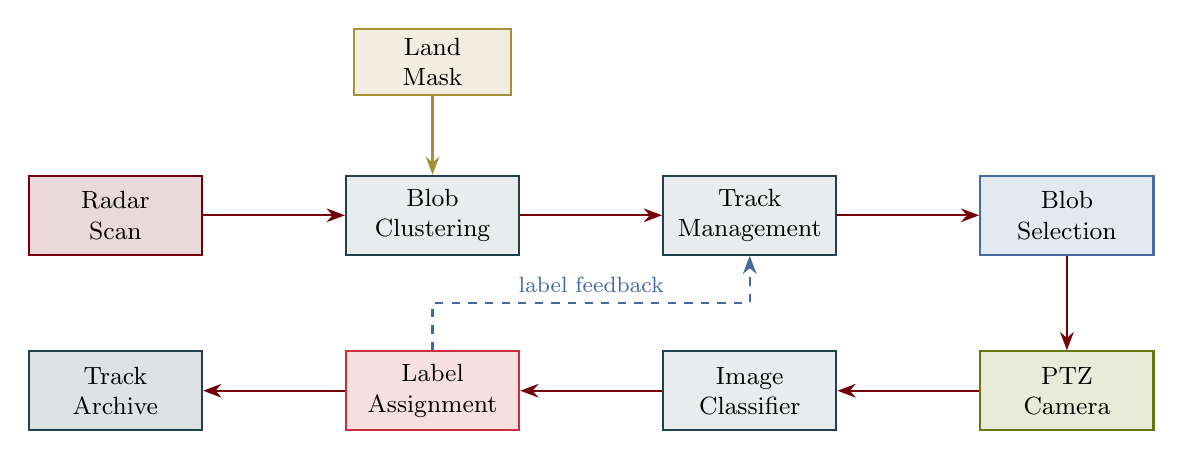
\begin{tikzpicture}[node distance=1.6cm and 1.8cm]
    % Nodes
    \node[sysblock, fill=Garnet!15, draw=Garnet] (radar) {Radar\\Scan};
    \node[sysblock, right=of radar] (cluster) {Blob\\Clustering};
    \node[sysblock, right=of cluster] (track) {Track\\Management};
    \node[sysblock, right=of track, fill=Atlantic!15, draw=Atlantic] (select) {Blob\\Selection};
    \node[sysblock, below=1.2cm of select, fill=Horseshoe!15, draw=Horseshoe] (camera) {PTZ\\Camera};
    \node[sysblock, left=of camera] (classify) {Image\\Classifier};
    \node[sysblock, left=of classify, fill=Rose!15, draw=Rose] (label) {Label\\Assignment};
    \node[sysblock, left=of label, fill=Congaree!15] (archive) {Track\\Archive};

    % Arrows
    \draw[sysarrow] (radar) -- (cluster);
    \draw[sysarrow] (cluster) -- (track);
    \draw[sysarrow] (track) -- (select);
    \draw[sysarrow] (select) -- (camera);
    \draw[sysarrow] (camera) -- (classify);
    \draw[sysarrow] (classify) -- (label);
    \draw[sysarrow] (label) -- (archive);

    % Feedback loop
    \draw[sysarrow, Atlantic, dashed] (label.north) -- ++(0,0.6) -| node[above, pos=0.25, font=\footnotesize, text=Atlantic] {label feedback} (track.south);

    % Land mask input
    \node[sysblock, above=1.0cm of cluster, fill=Honeycomb!15, draw=Honeycomb, minimum width=2.0cm, minimum height=0.7cm] (landmask) {Land\\Mask};
    \draw[sysarrow, Honeycomb] (landmask) -- (cluster);
\end{tikzpicture}
\end{document}
